%! TeX program = lualatex
\documentclass[main]{subfiles}

\begin{document}

\title[AutoML: BO]{Posterior Uncertainty and Acquisition Functions I}
\subtitle{Bayesian Surrogate Models and Lower Confidence Bound}
\author[Bernd Bischl]{Bernd Bischl}
\date{}

\titlebackground*{images/AutoML_HPO_2_2}

%\institute{}
%\date{}

    \maketitle


\begin{frame}{Bayesian Surrogate Modeling}
    \textbf{Goal:} Find a trade-off between \textbf{exploration} (areas we have not visited yet) and \textbf{exploitation} (search around good design points).
    \vfill
    \begin{center}
        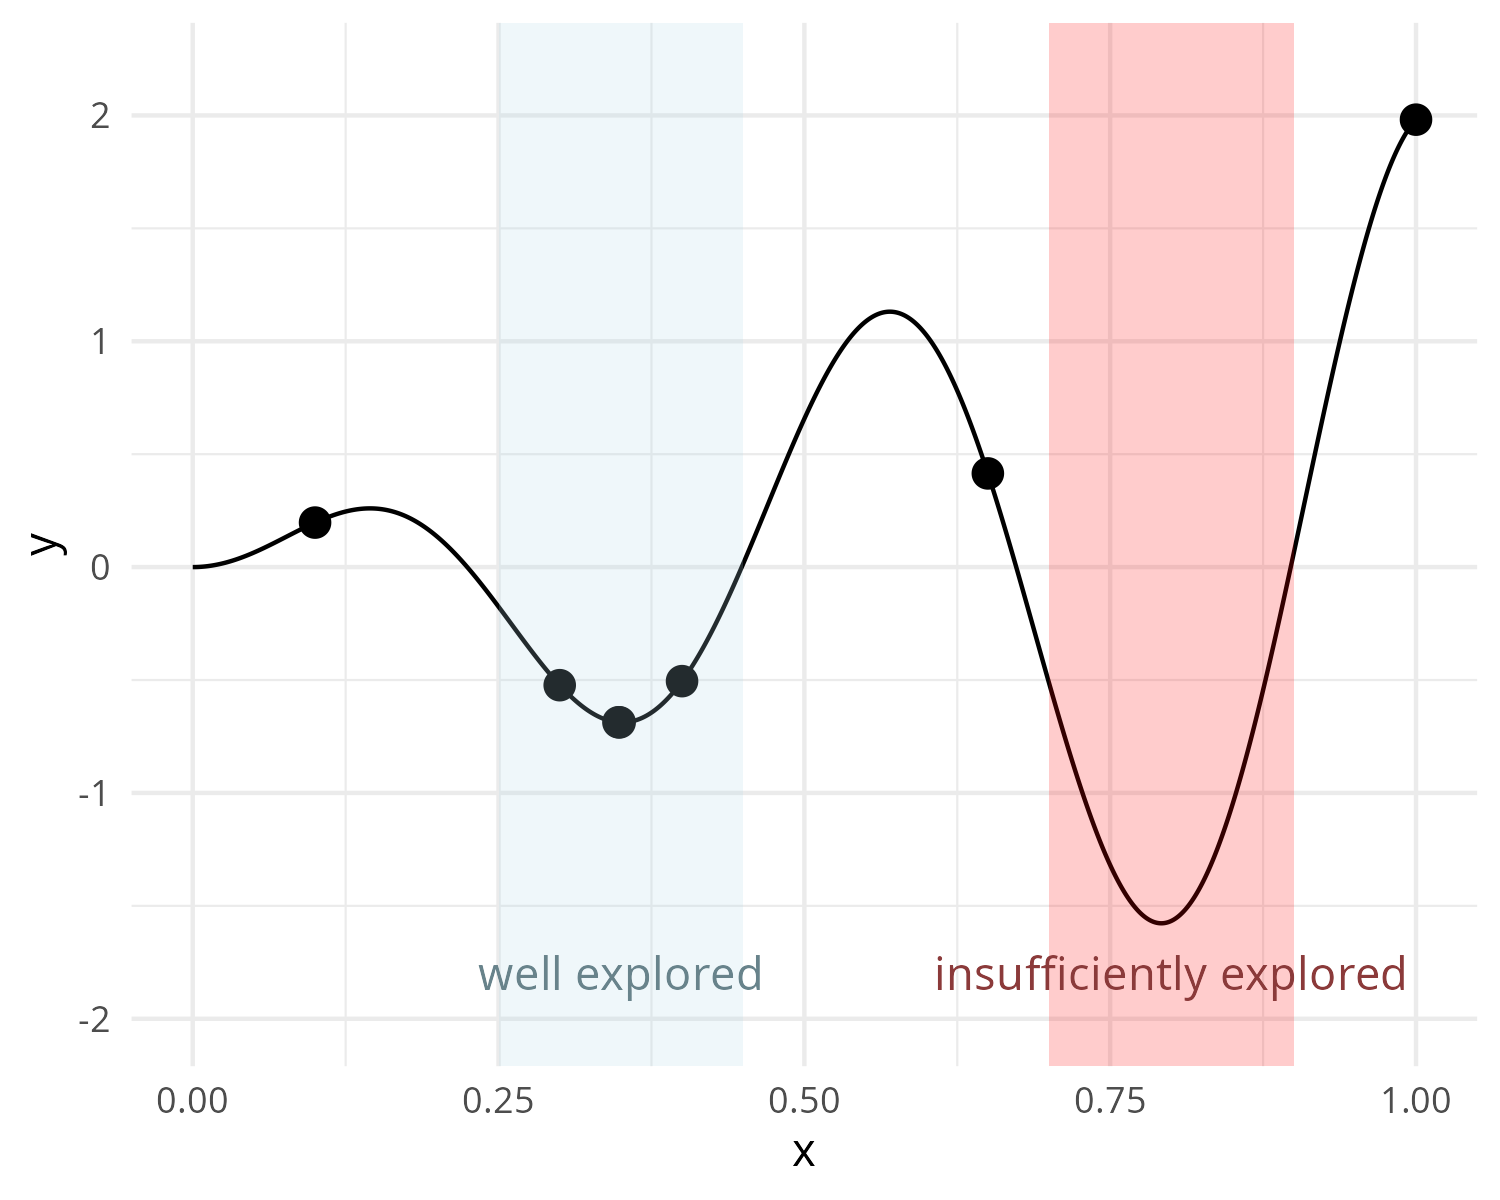
\includegraphics[width=.7\textwidth]{images/bayesian_loop_ee.png}
    \end{center}
\end{frame}


\begin{frame}{Bayesian Surrogate Modeling}
    \begin{itemize}
        \item \textbf{Idea:} Use a \textbf{Bayesian approach} to build a surrogate model yielding estimates for the posterior mean $\surro(\conf)$ and posterior variance $\sh^2(\conf)$
        \item $\sh^2(\conf)$ expresses ``confidence''/``certainty'' in the prediction
    \end{itemize}
    \vfill
    \begin{columns}[onlytextwidth]
        \column{.5\textwidth}
        \begin{center}
            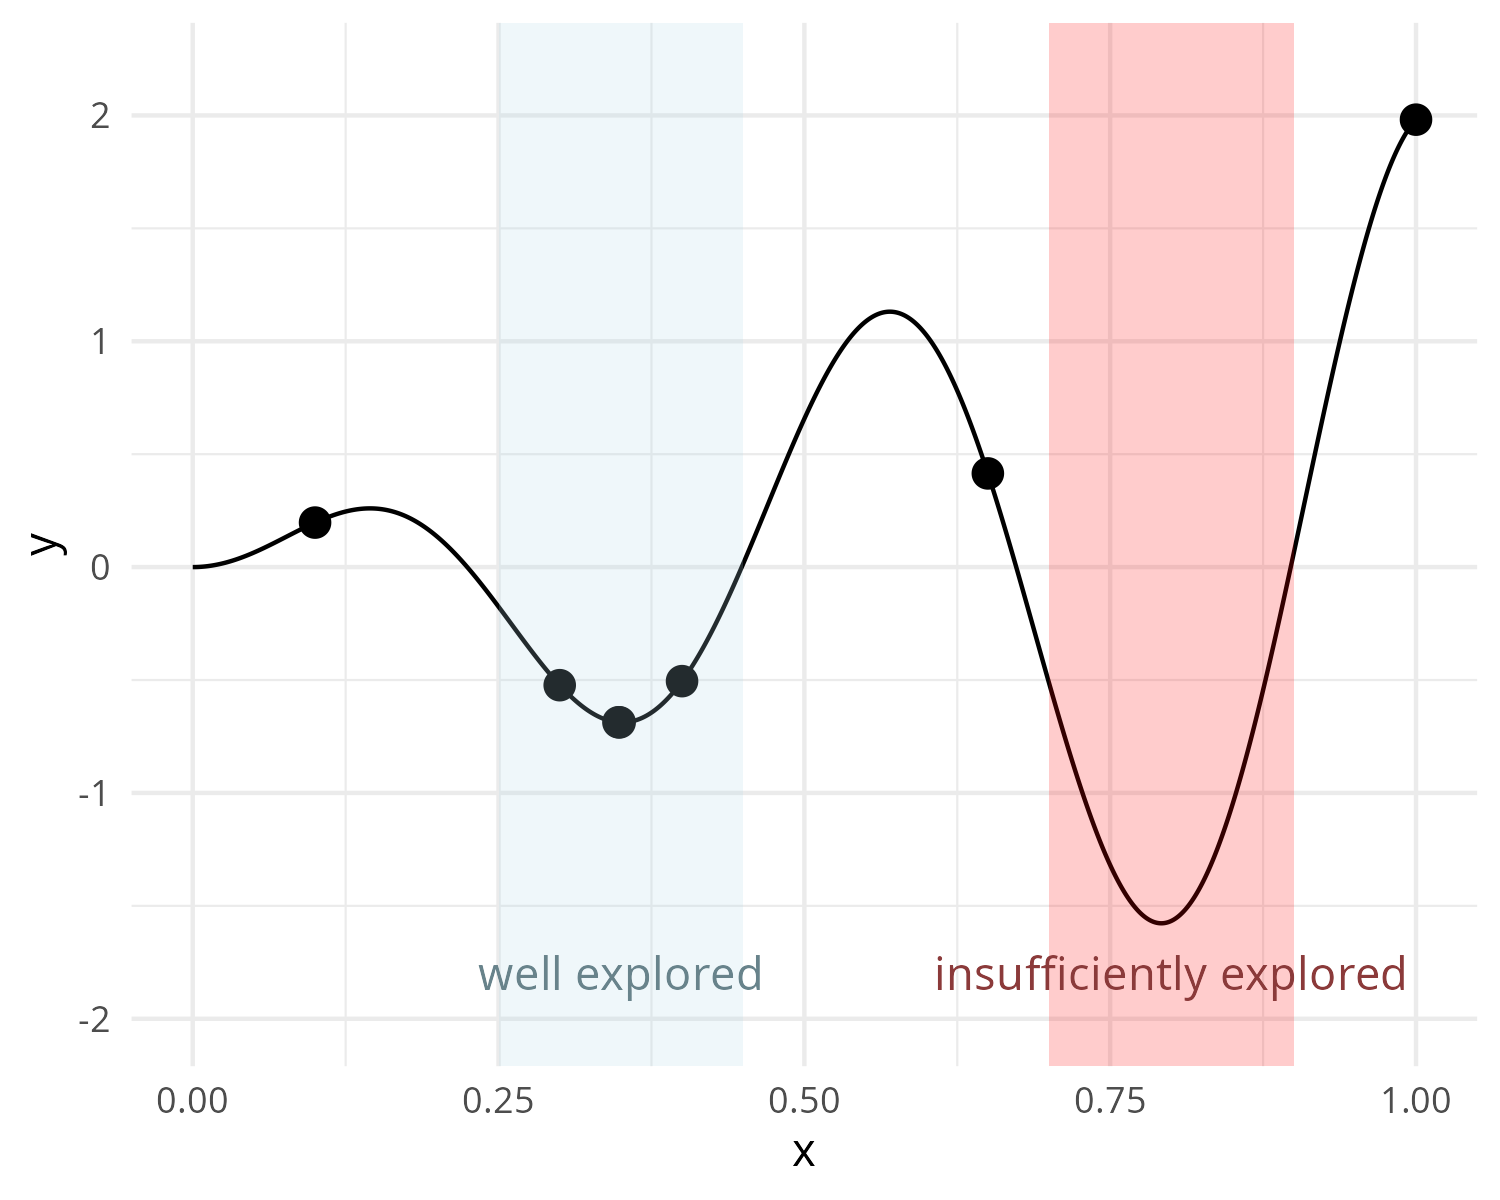
\includegraphics[width=\textwidth]{images/bayesian_loop_ee.png}
        \end{center}
        \column{.5\textwidth}
        \begin{center}
            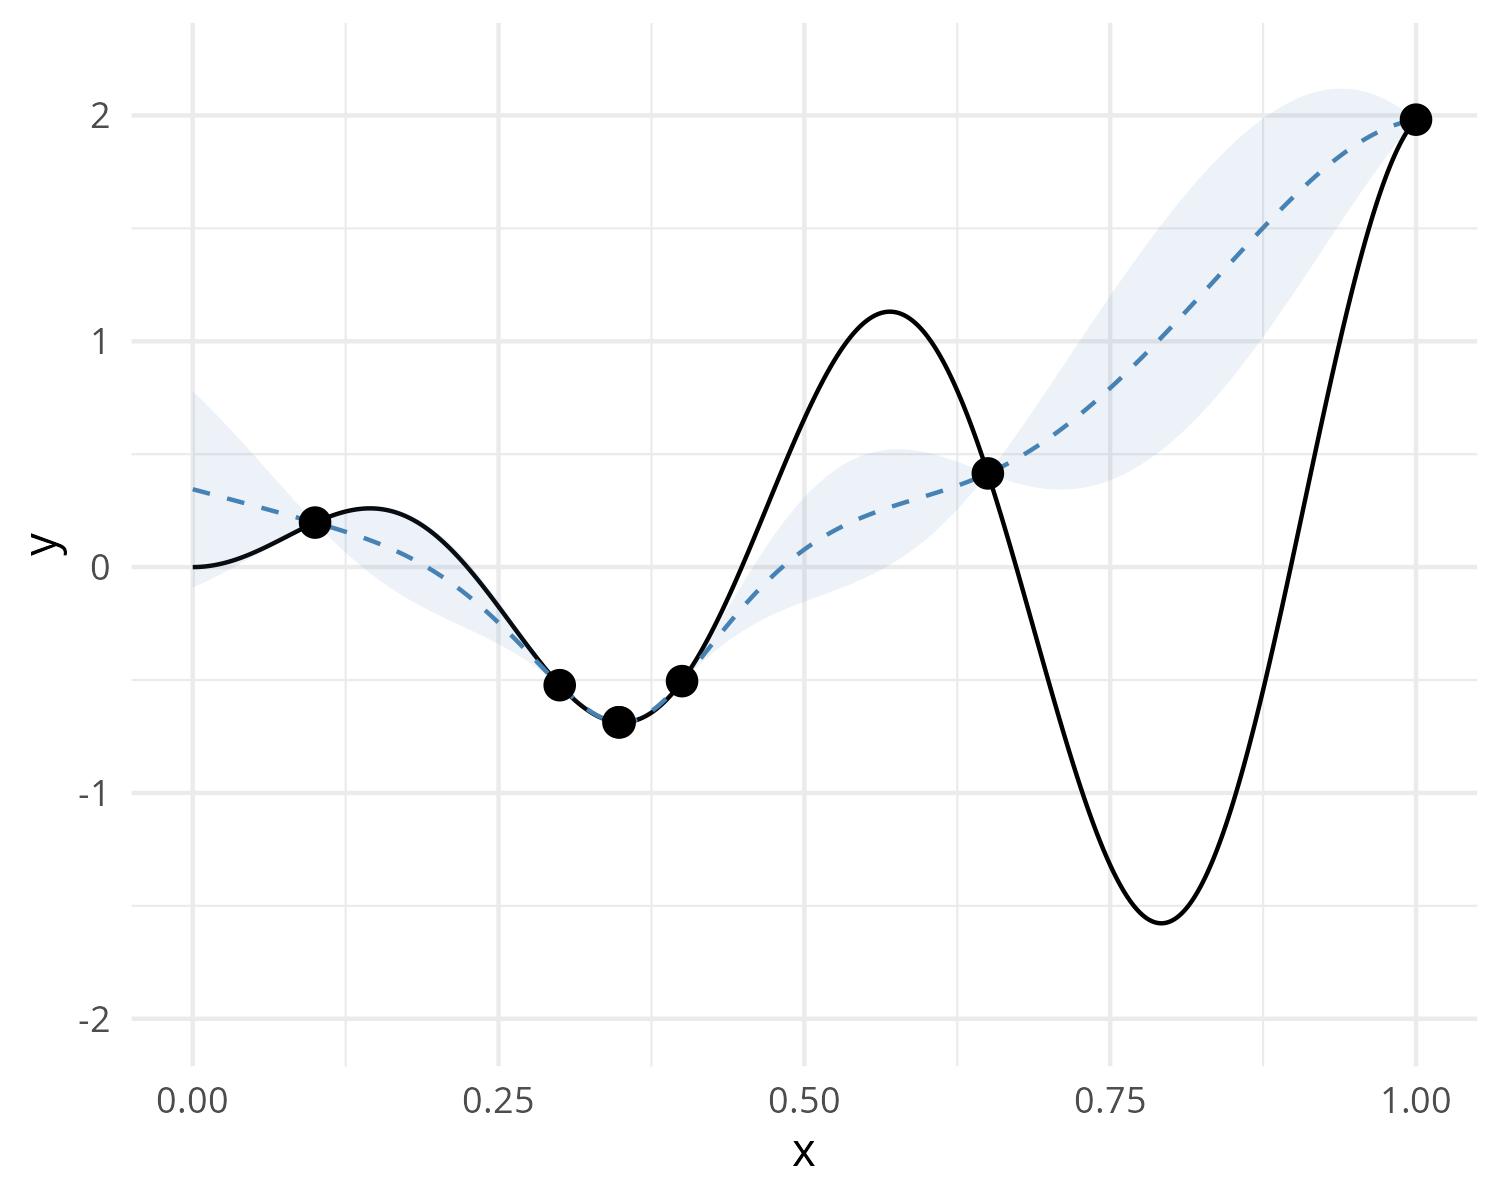
\includegraphics[width=\textwidth]{images/bayesian_loop_sm.png}
        \end{center}
    \end{columns}
\end{frame}


\begin{frame}{Bayesian Surrogate Modeling}
    \begin{itemize}
        \item Denote by $Y \mid \conf, \Dt$ the (conditional) random variable associated with the posterior predictive distribution of a new point $\conf$ under the surrogate model; abbreviated $Y(\conf)$
        \item Most prominent choice: a \textbf{Gaussian process}, here $Y(\conf) \sim \normal\left(\surro(\conf), \sh^2(\conf)\right)$
    \end{itemize}
    \vfill
    \begin{center}
        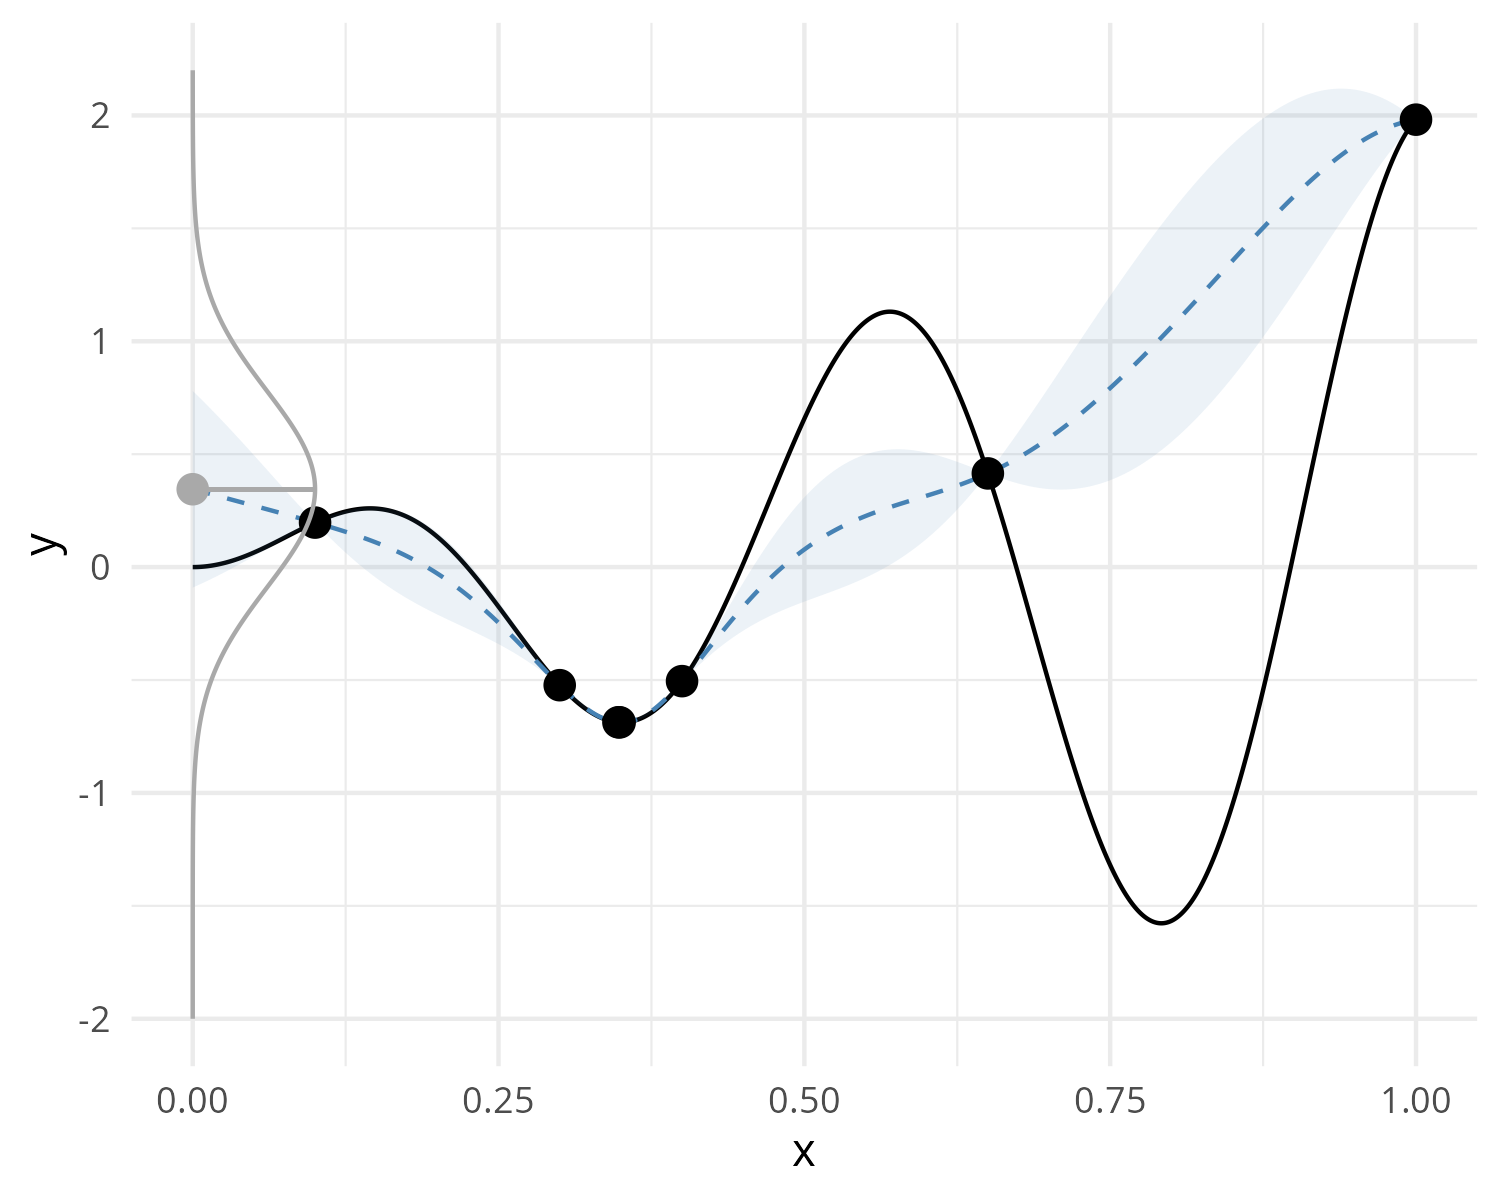
\includegraphics[width=.5\textwidth]{images/bayesian_loop_sm_normal.png}
    \end{center}
    \begin{footnotesize}
        For now we assume an interpolating SM; $\surro(\conf) = \cost(\conf)$ and $\sh(\conf) = 0$ at training points.
    \end{footnotesize}
\end{frame}


\begin{frame}{Acquisition Functions}
    To sequentially propose new points based on the surrogate model, we make use of so-called acquisition functions $a: \pcs \to \R$.
    \vfill
    Let $\fmin := \min\{\cost(\confI{1}), \ldots, \cost(\confI{t})\}$ denote the best observed value so far (visualized in green).
    \begin{center}
        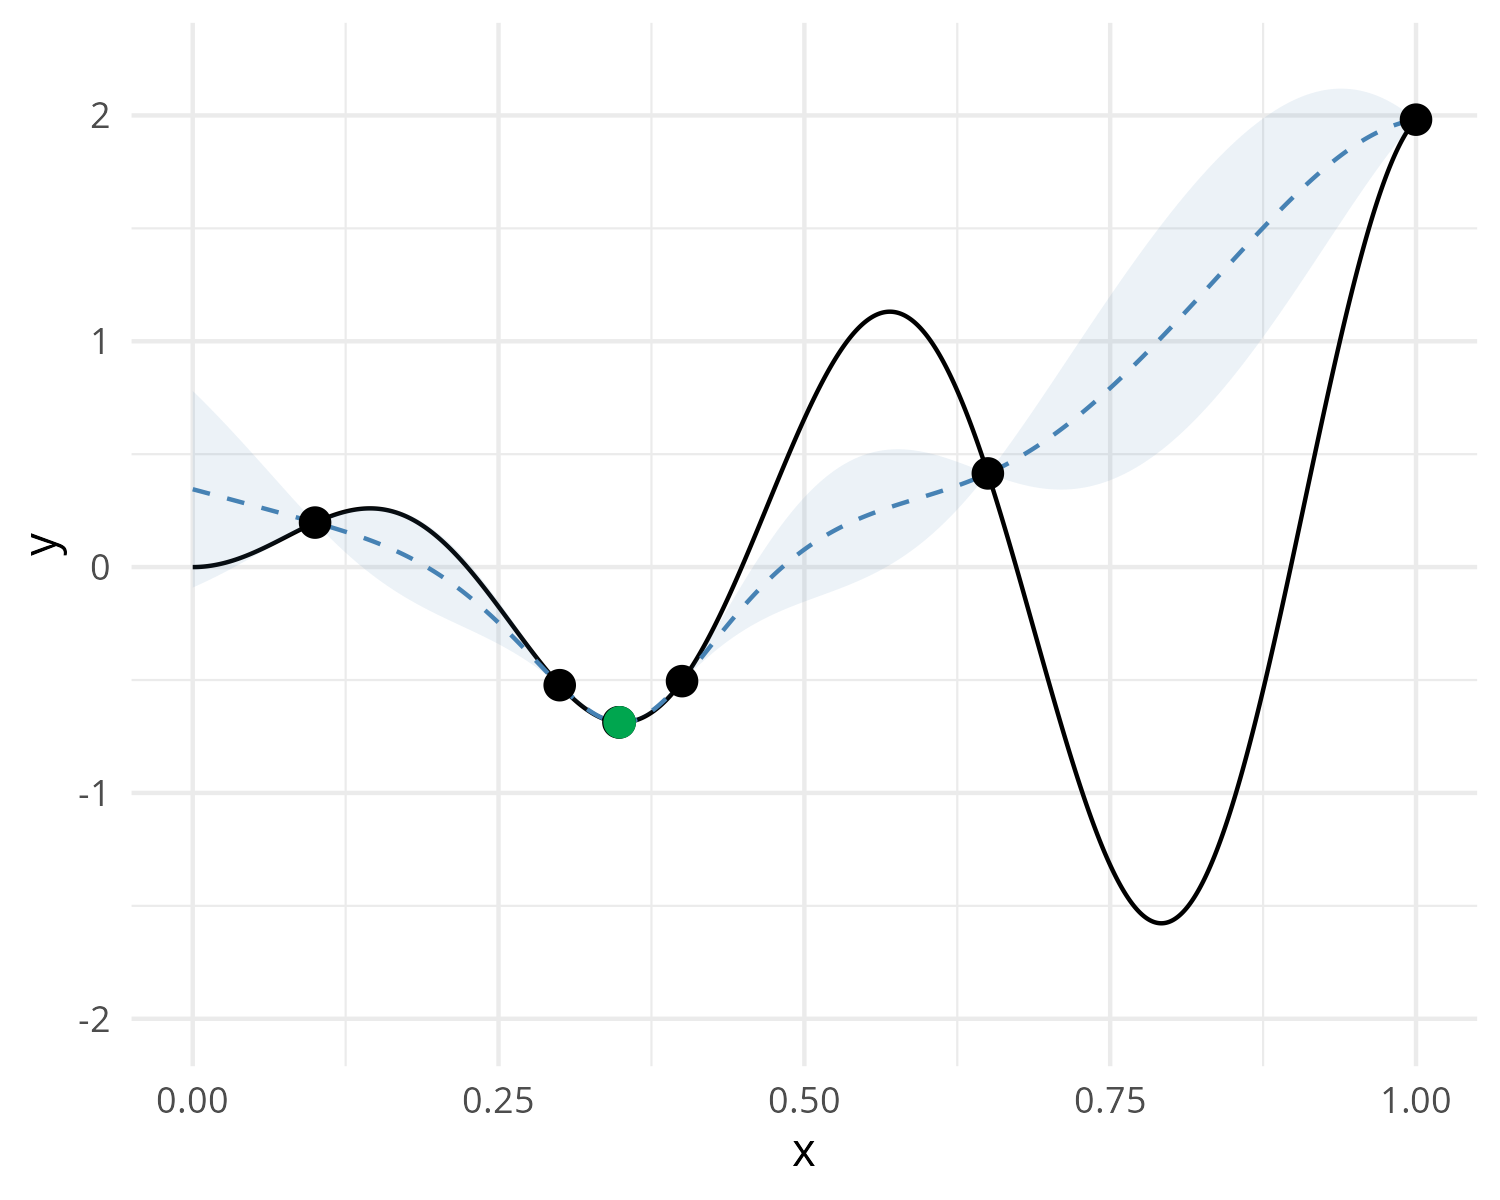
\includegraphics[width=.5\textwidth]{images/bayesian_loop_sm_fmin.png}
    \end{center}
    In the examples before, we simply used the posterior mean $a(\conf) = \surro(\conf)$ as acquisition function -- ignoring uncertainty.
\end{frame}


\begin{frame}{Lower Confidence Bound}
    \textbf{Goal:} Find $\confI{t+1}$ that minimizes the \textbf{Lower Confidence Bound} (LCB):
    $$a_{\text{LCB}}(\conf) = \surro(\conf) - \tau \sh(\conf)$$
    where $\tau > 0$ is a constant that controls the ``mean vs.\ uncertainty'' trade-off.
    \vfill
    The LCB is conceptually very simple and does \textbf{not} rely on distributional assumptions on the posterior predictive distribution.
\end{frame}


\begin{frame}{Lower Confidence Bound}
    $\tau = 1$
    \vfill
    \begin{center}
        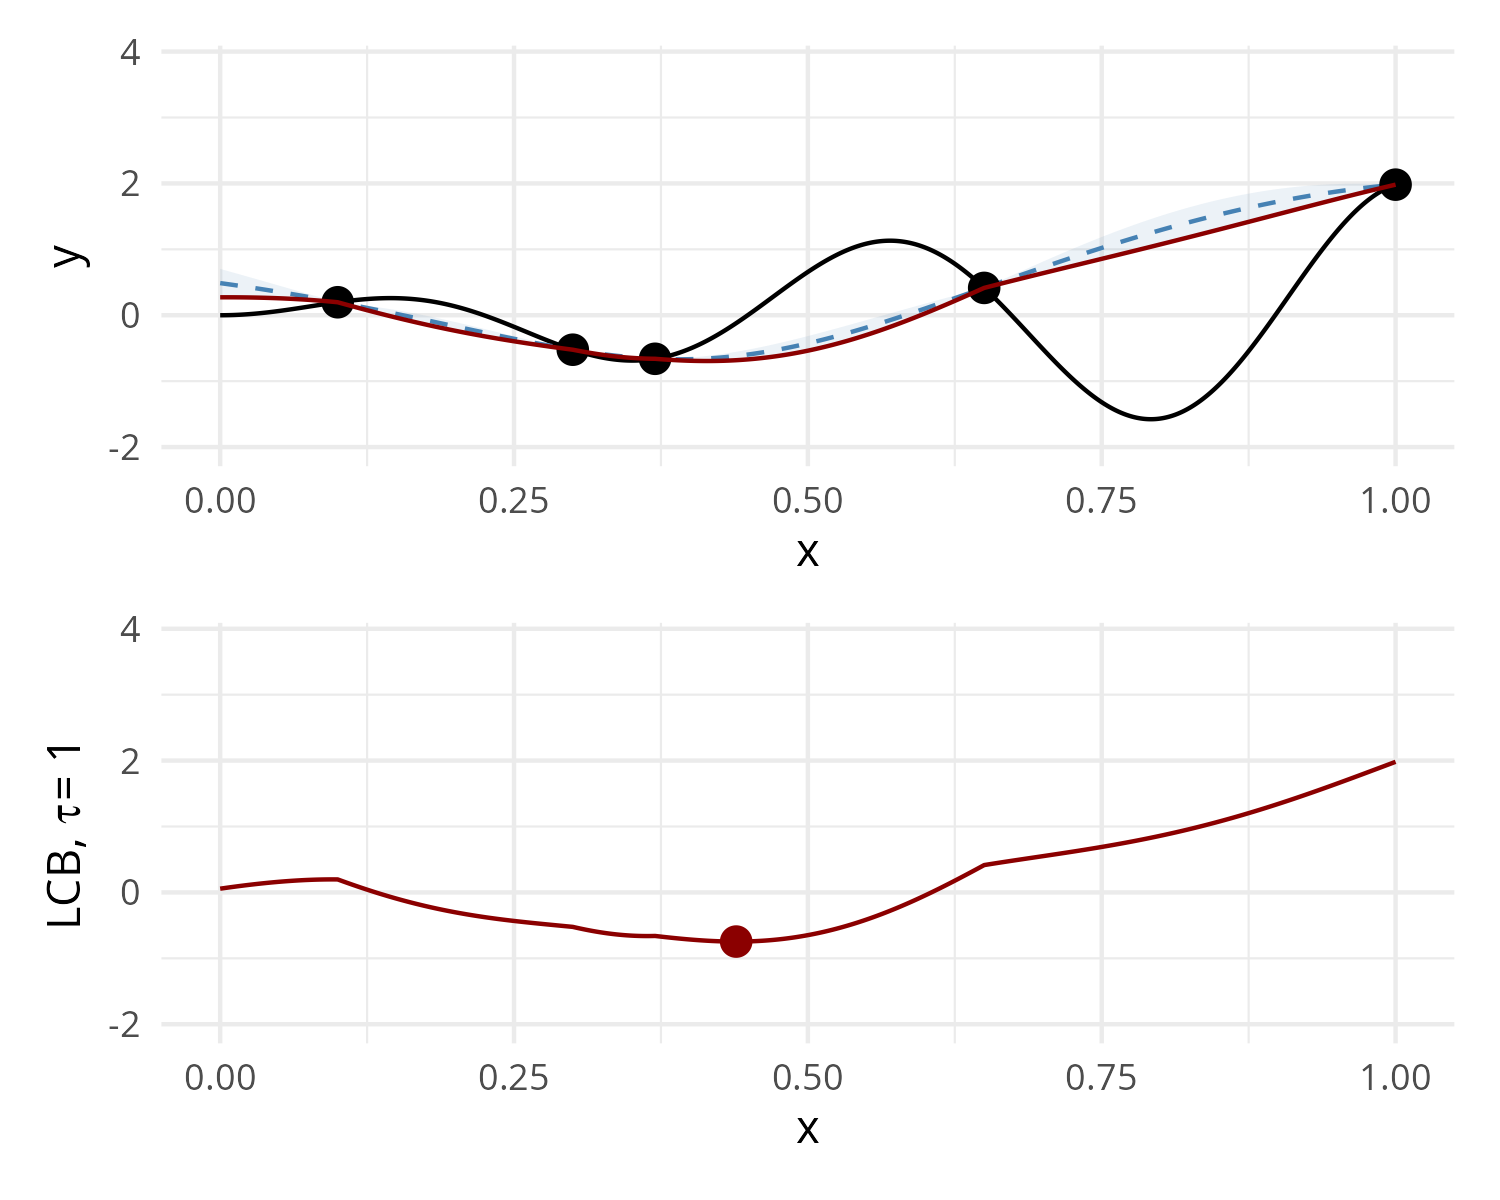
\includegraphics[width=.7\textwidth]{images/bayesian_loop_lcb_0.png}
    \end{center}
    \vfill
    Top: Design points and surrogate model showing $\surro(\conf)$ (blue) and $\surro(\conf) - \tau \sh(\conf)$ (red).\\
    Bottom: The red point depicts $\argmin_{\conf \in \pcs} a_{\text{LCB}}(\conf)$.
\end{frame}


\begin{frame}{Lower Confidence Bound}
    $\tau = 5$
    \vfill
    \begin{center}
        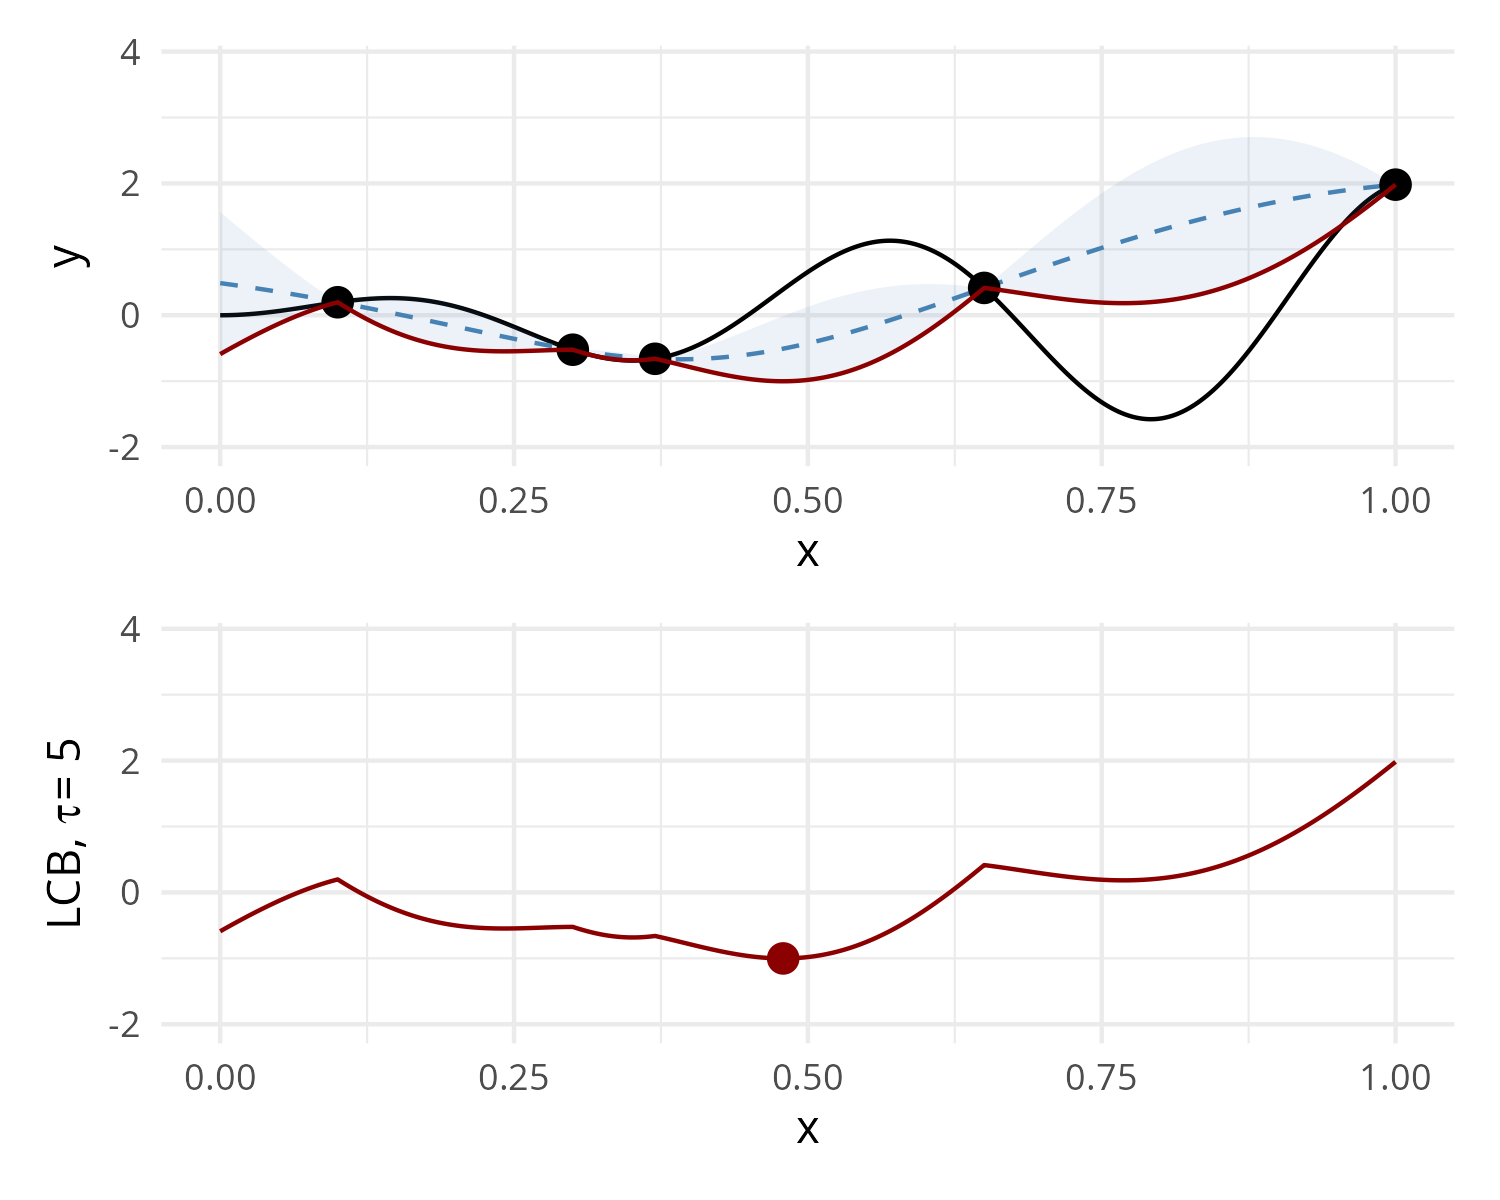
\includegraphics[width=.7\textwidth]{images/bayesian_loop_lcb_1.png}
    \end{center}
\end{frame}


\begin{frame}{Lower Confidence Bound}
    $\tau = 10$
    \vfill
    \begin{center}
        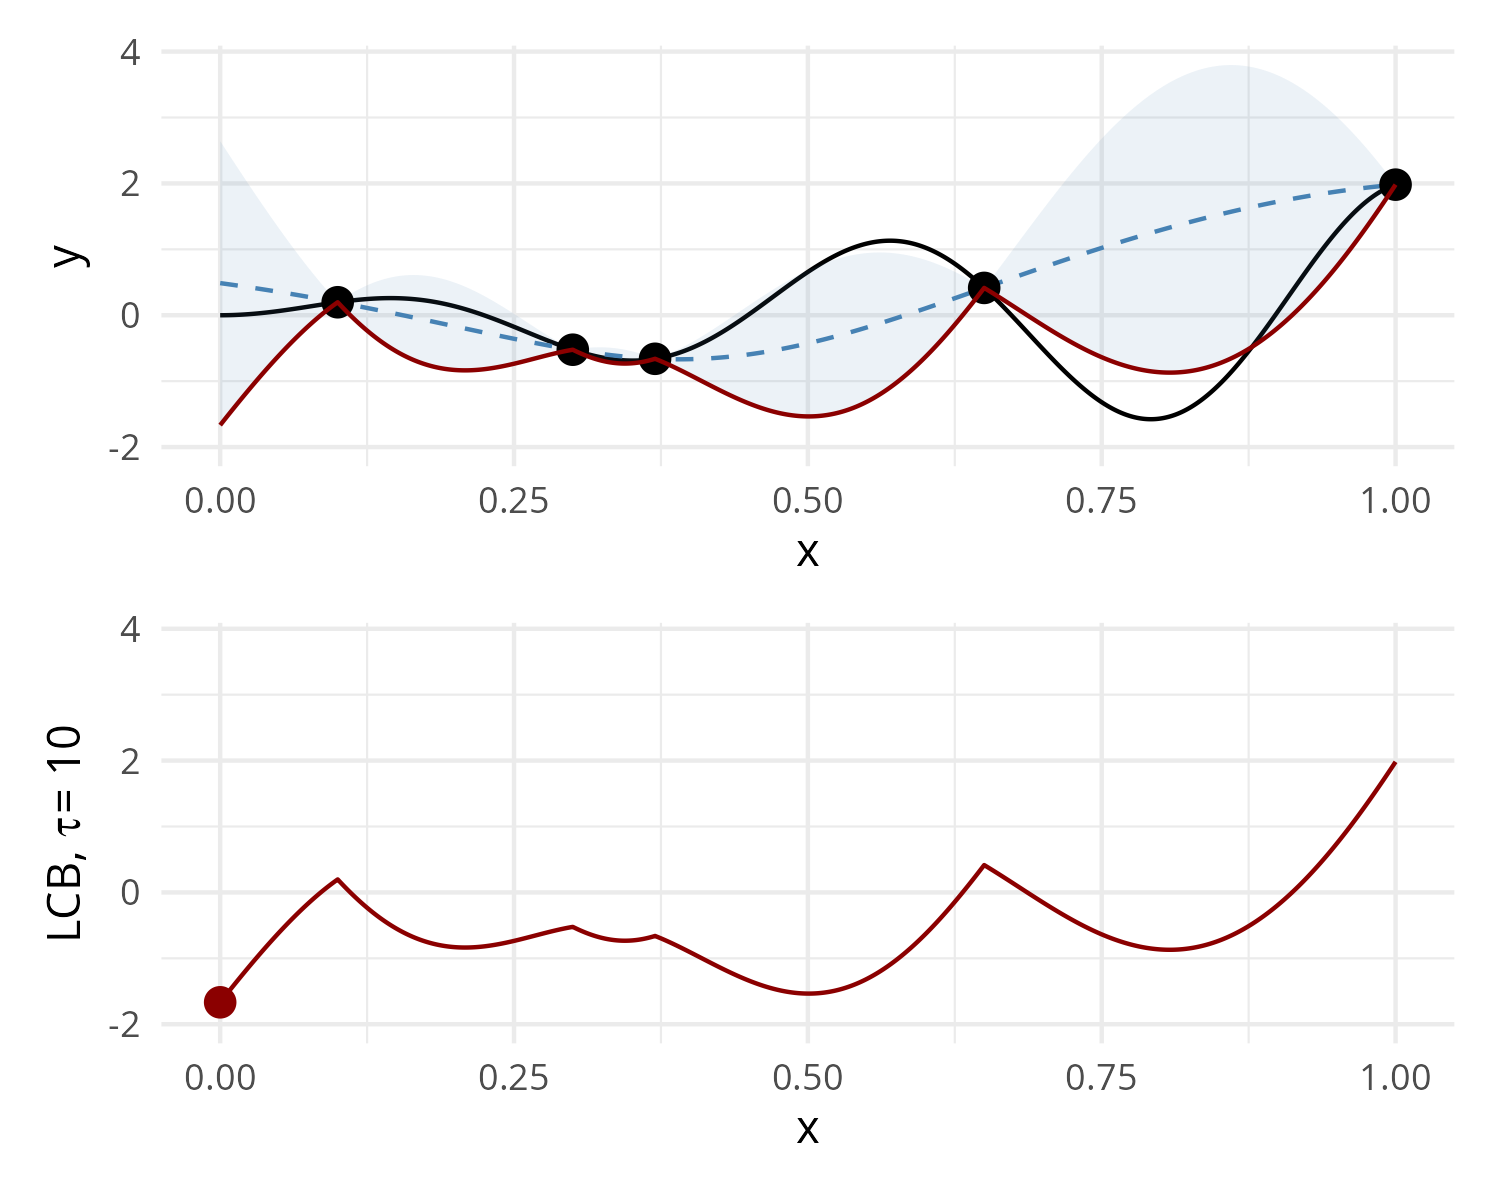
\includegraphics[width=.7\textwidth]{images/bayesian_loop_lcb_2.png}
    \end{center}
\end{frame}


\begin{frame}{Summary}
\begin{enumerate}
    \item Bayesian surrogate models provide both posterior mean and variance to trade off exploration and exploitation
    \item Gaussian processes are the most prominent choice
    \item The Lower Confidence Bound is a simple acquisition function with an explicit mean/uncertainty trade-off parameter $\tau$
\end{enumerate}
\end{frame}

\end{document}
